%% Presentación de avances de la Etapa 3 al profesor guía (28/10/2026).
%% Compilar desde esta carpeta: latexmk -pdf -outdir=build presentacion.tex
%% El único aviso esperado es «Overfull \vbox (15.6pt)» en la portada: lo da el tema metropolis incluso en un documento mínimo
%% (comprobado el 26/10/2026) y no se ve; cualquier otro Overfull se corrige.
%% Manda el informe: problema, objetivos y cifras se copian de informe-oficial/ y docs/ (la fuente va al pie de cada lámina).
%% Figuras: la arquitectura es la vista resumida de docs/10 §1 (generar-figuras.sh); el cableado se exporta de
%% plataforma/firmware/cableado-fase-1.drawio (sin fechas en los metadatos).
\documentclass[aspectratio=169,11pt]{beamer}
\usepackage[T1]{fontenc}
\usepackage[utf8]{inputenc}
\usepackage[spanish,es-noquoting]{babel}
\usepackage{booktabs}
\usepackage{array}
\newcolumntype{L}[1]{>{\raggedright\arraybackslash}p{#1}}
\usepackage{graphicx}
\usepackage{tcolorbox}
\tcbuselibrary{skins}
\usetheme[progressbar=frametitle,numbering=fraction,block=fill]{metropolis}
\usepackage{tgheros}
\renewcommand{\familydefault}{\sfdefault}
\graphicspath{{../figuras/render/}{../figuras/drawio/}{figuras/}}

%% Paleta: azul marino institucional y un acento turquesa; sobrio para una presentación formal.
\definecolor{marino}{HTML}{0B1F3A}
\definecolor{acento}{HTML}{0FA3B1}
\definecolor{suave}{HTML}{EEF3F7}
\definecolor{texto}{HTML}{1E2A36}
\definecolor{gris}{HTML}{6B7785}
\definecolor{bien}{HTML}{1F7A4D}
\definecolor{curso}{HTML}{B26A00}
\setbeamercolor{normal text}{fg=texto,bg=white}
\setbeamercolor{frametitle}{fg=white,bg=marino}
\setbeamercolor{progress bar}{fg=acento,bg=marino!70}
\setbeamercolor{title separator}{fg=acento}
\setbeamercolor{alerted text}{fg=acento}
\setbeamercolor{block title}{fg=marino,bg=suave}
\setbeamercolor{block body}{bg=suave!50}
\setbeamercolor{background canvas}{bg=white}
\setbeamercolor{standout text}{fg=white,bg=marino}
\setbeamerfont{frametitle}{size=\large,series=\bfseries}
\setbeamerfont{title}{size=\Large,series=\bfseries}
\setbeamerfont{subtitle}{size=\normalsize}
%% La fuente de cada lámina va en el pie (\fuente la deja y el pie la borra al imprimirla): nunca se superpone al contenido.
\gdef\lafuente{}
\setbeamertemplate{frame footer}{\ifx\lafuente\empty\else Fuente: \lafuente\fi\gdef\lafuente{}}
\setbeamerfont{page number in head/foot}{size=\scriptsize}
\setbeamercolor{footline}{fg=gris}

\newcommand{\fuente}[1]{\gdef\lafuente{#1}}
\newcommand{\hecho}{\textcolor{bien}{\textbf{Cumplido}}}
\newcommand{\encurso}{\textcolor{curso}{\textbf{En curso}}}
\newcommand{\avanzado}{\textcolor{curso}{\textbf{Avanzado}}}
%% Indicador: cifra grande y su etiqueta, en una tarjeta.
\newtcolorbox{tarjeta}[1][]{colback=suave,colframe=suave,arc=2pt,boxrule=0pt,left=6pt,right=6pt,top=5pt,bottom=5pt,
  halign=center,valign=center,#1}
\newcommand{\cifra}[2]{\begin{tarjeta}{\large\bfseries\color{marino}#1}\\[1pt]{\scriptsize\color{gris}#2}\end{tarjeta}}

\title{Sistema integrado para el registro, gestión y monitoreo de dispositivos IoT}
\subtitle{Etapa 3: mejoras, pruebas adicionales y validación preliminar}
\author{Vicente Ricardo Ramírez Oñate}
\institute{INFO-1197 · Universidad Católica de Temuco · Profesor guía: Mario Villanueva}
\date{5 de noviembre de 2026}

\begin{document}

\maketitle

\begin{frame}{En una frase}
  \vfill
  \begin{tarjeta}[halign=left,left=14pt,right=14pt,top=12pt,bottom=12pt,borderline west={3pt}{0pt}{acento}]
    \large El núcleo del sistema funciona de punta a punta con dispositivos reales, está medido y probado, y cabe en una
    fracción de la memoria que pide el referente (ThingsBoard, 4~GB).
  \end{tarjeta}
  \medskip
  La Etapa 4 está planificada en orden y con sus horas.
  \vfill
\end{frame}

\begin{frame}{El problema y el objetivo general}
  \begin{block}{Problema}
    La Facultad de Ingeniería no puede consultar fácilmente, en un solo lugar, los datos de sensores de distinto origen:
    cada fabricante entrega su propia plataforma y la información queda repartida.
  \end{block}
  \footnotesize
  Cinco causas: formatos distintos, plataforma atada al equipo, costo y datos en la nube del fabricante, sin personal
  dedicado, y el silencio de un dispositivo que no se distingue de la falta de novedades.
  \normalsize
  \begin{block}{Objetivo general}
    Desarrollar un prototipo de sistema integrado para el registro, gestión y monitoreo en tiempo real de dispositivos IoT,
    con un \emph{dashboard} que centralice sus datos, estado y alertas, para su aprovechamiento en la investigación de la
    Facultad.
  \end{block}
  \fuente{informe, capítulo 1 (problema central y objetivo general)}
\end{frame}

\begin{frame}{Objetivos específicos}
  \footnotesize
  \begin{tabular}{@{}L{0.53\linewidth}L{0.12\linewidth}L{0.28\linewidth}@{}}
    \toprule
    \textbf{Objetivo} & \textbf{Plazo} & \textbf{Estado} \\
    \midrule
    \textbf{OE1} Caracterizar las necesidades de la Facultad: literatura, oferta y entrevistas & 30/10 & \hecho: dos
      entrevistas (05/10 y 25/10) \\
    \textbf{OE2} Evaluar y seleccionar el transporte y el formato de los datos & 02/10 & \hecho: MQTT y SenML \\
    \textbf{OE3} Diseñar la arquitectura, el modelo de datos y el despliegue & 02/10 & \hecho: cinco alojamientos
      comparados \\
    \textbf{OE4} Implementar: núcleo mínimo con un dispositivo real (30/10); registro, alertas y \emph{dashboard} (04/12)
      & 30/10 y\newline 04/12 & \encurso: núcleo 25 de 34 tareas \\
    \textbf{OE5} Validar en un servidor modesto contra los umbrales de los requerimientos & 04/12 & Etapa 4; mediciones
      preliminares hechas \\
    \bottomrule
  \end{tabular}
  \fuente{informe, capítulo 1 (objetivos); docs/18 §1}
\end{frame}

\begin{frame}{Arquitectura: el recorrido de una trama}
  \centering
  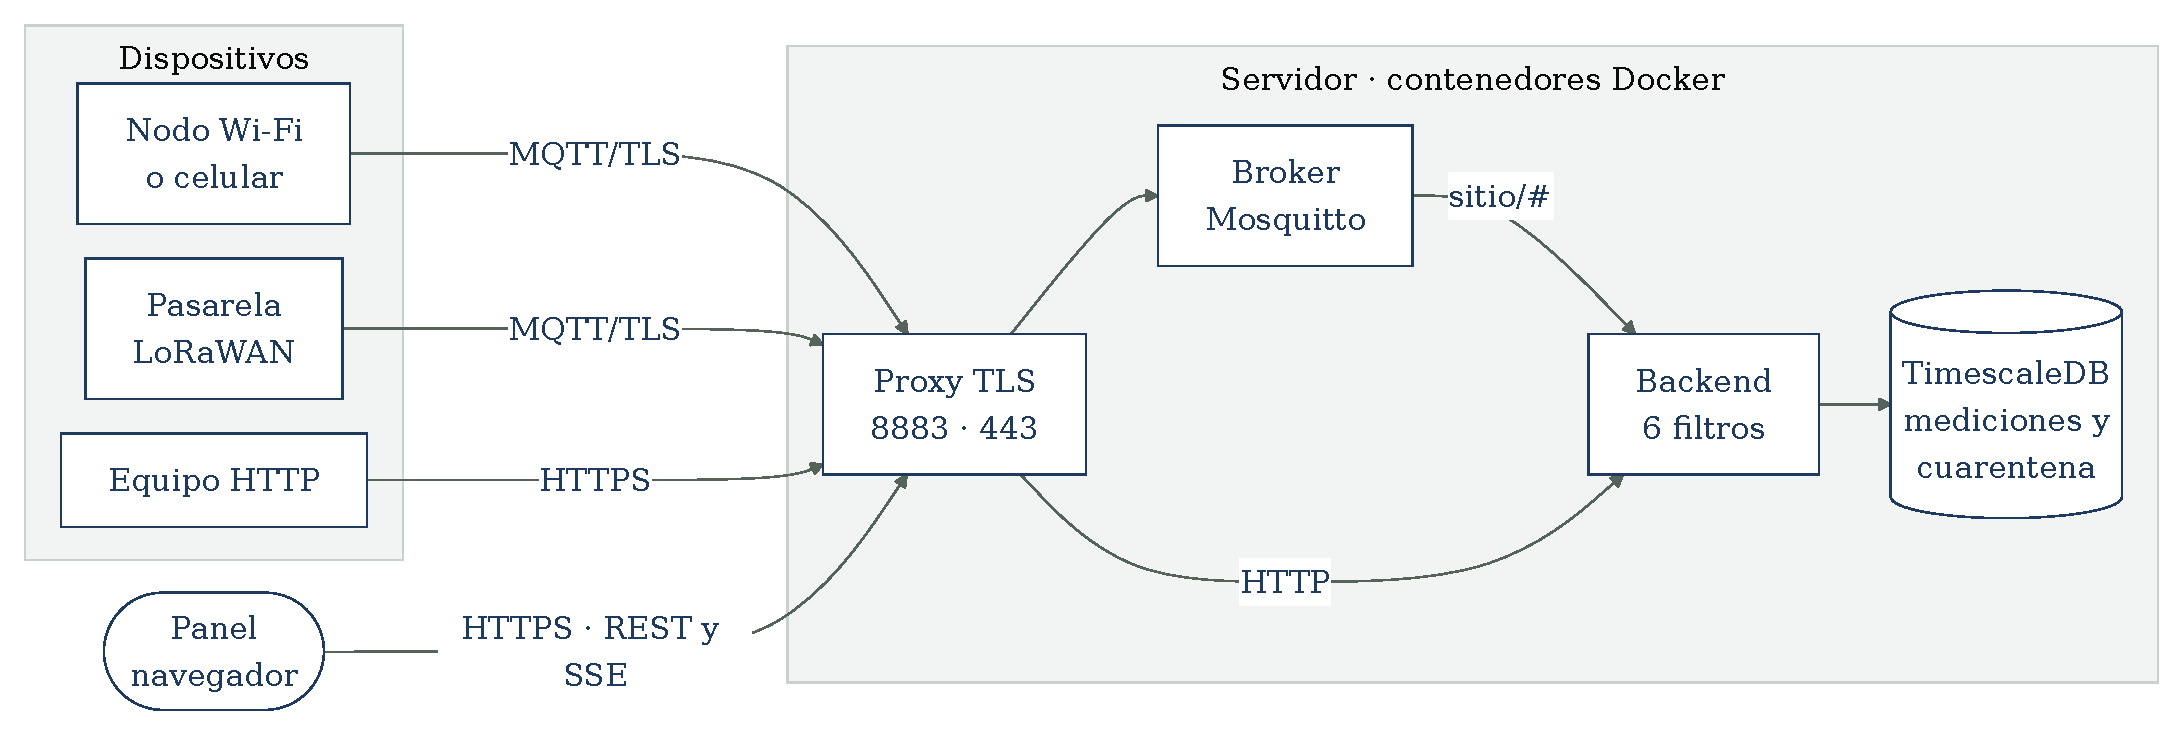
\includegraphics[width=\linewidth,height=0.56\textheight,keepaspectratio]{resumen.pdf}
  \smallskip
  \begin{columns}[T,onlytextwidth]
    \begin{column}{0.31\textwidth}{\scriptsize Las vías 1 a 3 entran cifradas por un solo
      \textbf{proxy TLS}; el backend es el \textbf{único que lee los datos} (\texttt{sitio/\#}).\par}\end{column}
    \begin{column}{0.31\textwidth}{\scriptsize \textbf{Seis filtros}: autenticar,
      analizar, validar, normalizar, alertar y supervisar.\par}\end{column}
    \begin{column}{0.31\textwidth}{\scriptsize Contrato \textbf{SenML}; lo rechazado va
      a \textbf{cuarentena con su motivo}.\par}\end{column}
  \end{columns}
  \fuente{docs/10 §1 (vista resumida y vista de contenedores)}
\end{frame}

\begin{frame}{Cómo llega una trama: vías y rutas LoRaWAN}
  \begin{columns}[T,onlytextwidth]
    \begin{column}{0.49\textwidth}
      {\small\textbf{Vías}: por dónde viaja la trama}\par\smallskip
      \scriptsize
      \begin{tabular}{@{}L{0.55\linewidth}L{0.36\linewidth}@{}}
        \toprule
        Vía & Probada \\
        \midrule
        1. MQTT/TLS (8883): nodo directo & ESP32, 24 h \\
        1. MQTT/TLS (8883): pasarela LoRaWAN, ruta B & UG65 del campus, 20/10 \\
        2. HTTPS (443): equipo directo & 04/11 con TLS; banco 180/180 \\
        2. \textit{Prevista:} pasarela por HTTPS (443) & Etapa 4 \\
        3. \textit{Diseñada:} WebSocket/TLS (443), Basics Station, ruta A & Etapa 4 (it. 2) \\
        \bottomrule
      \end{tabular}
    \end{column}
    \begin{column}{0.49\textwidth}
      {\small\textbf{Rutas LoRaWAN}: dónde está el servidor}\par\smallskip
      \scriptsize
      \begin{tabular}{@{}L{0.16\linewidth}L{0.76\linewidth}@{}}
        \toprule
        Ruta & Servidor de red \\
        \midrule
        B & Embebido en la pasarela (UG65, la red del campus hoy): \textbf{probada en campo} \\
        C & Servidor de red externo (p. ej. un ChirpStack institucional, por confirmar): formato probado en el banco \\
        A & ChirpStack propio en nuestro servidor: opcional \\
        \bottomrule
      \end{tabular}
    \end{column}
  \end{columns}
  \footnotesize La 2 la envía el propio equipo, con su token y en SenML, o la pasarela en nombre de sus nodos, con su JSON (prevista).\\
Las rutas B y C entran igual por la vía 1; solo cambia el adaptador.
  \fuente{docs/10 §1 (vías dibujadas y rutas); docs/16 §45, §49 y §53}
\end{frame}

\begin{frame}{Cómo se trabajó}
  \begin{columns}[T,onlytextwidth]
    \begin{column}{0.62\textwidth}
      \begin{itemize}
        \item El diseño escrito manda: primero \texttt{docs/}, después el código.
        \item Un \textbf{guardián} comprueba que documentos, código, base e informe digan lo mismo.
        \item \textbf{Banco de pruebas desechable}: se levanta desde cero y se borra al apagar.
        \item Cada control se prueba \textbf{plantando la falla}.
        \item \textbf{Revisión independiente} al cerrar cada bloque; cada hallazgo se verifica antes de corregir.
      \end{itemize}
    \end{column}
    \begin{column}{0.33\textwidth}
      \cifra{357}{pruebas automáticas del backend}
      \cifra{107}{pruebas del panel}
      \cifra{47}{pasos del guardián}
    \end{column}
  \end{columns}
  \fuente{plataforma/pruebas/verificar-todo.sh; docs/18 §1}
\end{frame}

\begin{frame}{Prueba de campo: red LoRaWAN del campus (20/10)}
  \begin{columns}[T,onlytextwidth]
    \begin{column}{0.3\textwidth}
      \cifra{813}{mediciones en 3 h}
      \cifra{2}{nodos (uno con sensor real) y una pasarela real, por TLS}
    \end{column}
    \begin{column}{0.66\textwidth}
      \textbf{Dos hallazgos reales, mostrados por el sistema y corregidos, y una respuesta sola:}
      \begin{enumerate}
        \item Reloj de la pasarela \textbf{4 días atrasado} $\to$ tolerancia de 10 min y condición «reloj desviado».
        \item Tópico \texttt{\$devEUI} sin resolver $\to$ cuarentena; plantilla del alta corregida.
        \item 27 min sin reenvío (operación) $\to$ «sin comunicación» a los 6 min, cerrada sola.
      \end{enumerate}
      \medskip
      \small El operador de la red, entrevistado después, pidió primero estado y alertas, después calidad del enlace, y
      alta masiva por archivo.
    \end{column}
  \end{columns}
  \fuente{docs/16 §45 y §46; bitácora de la entrevista del 25/10}
\end{frame}

\begin{frame}{El nodo propio: ESP32 con tres sensores}
  \begin{columns}[c,onlytextwidth]
    \begin{column}{0.3\textwidth}
      \footnotesize
      \begin{itemize}
        \item Aire (BME280), suelo (capacitivo) y sonda de temperatura (DS18B20).
        \item Wi-Fi y MQTT con TLS, cada 60 s, con credencial y tópico propios.
        \item Se cablea sin corriente y se revisa antes de conectar.
      \end{itemize}
    \end{column}
    \begin{column}{0.68\textwidth}
      \centering
      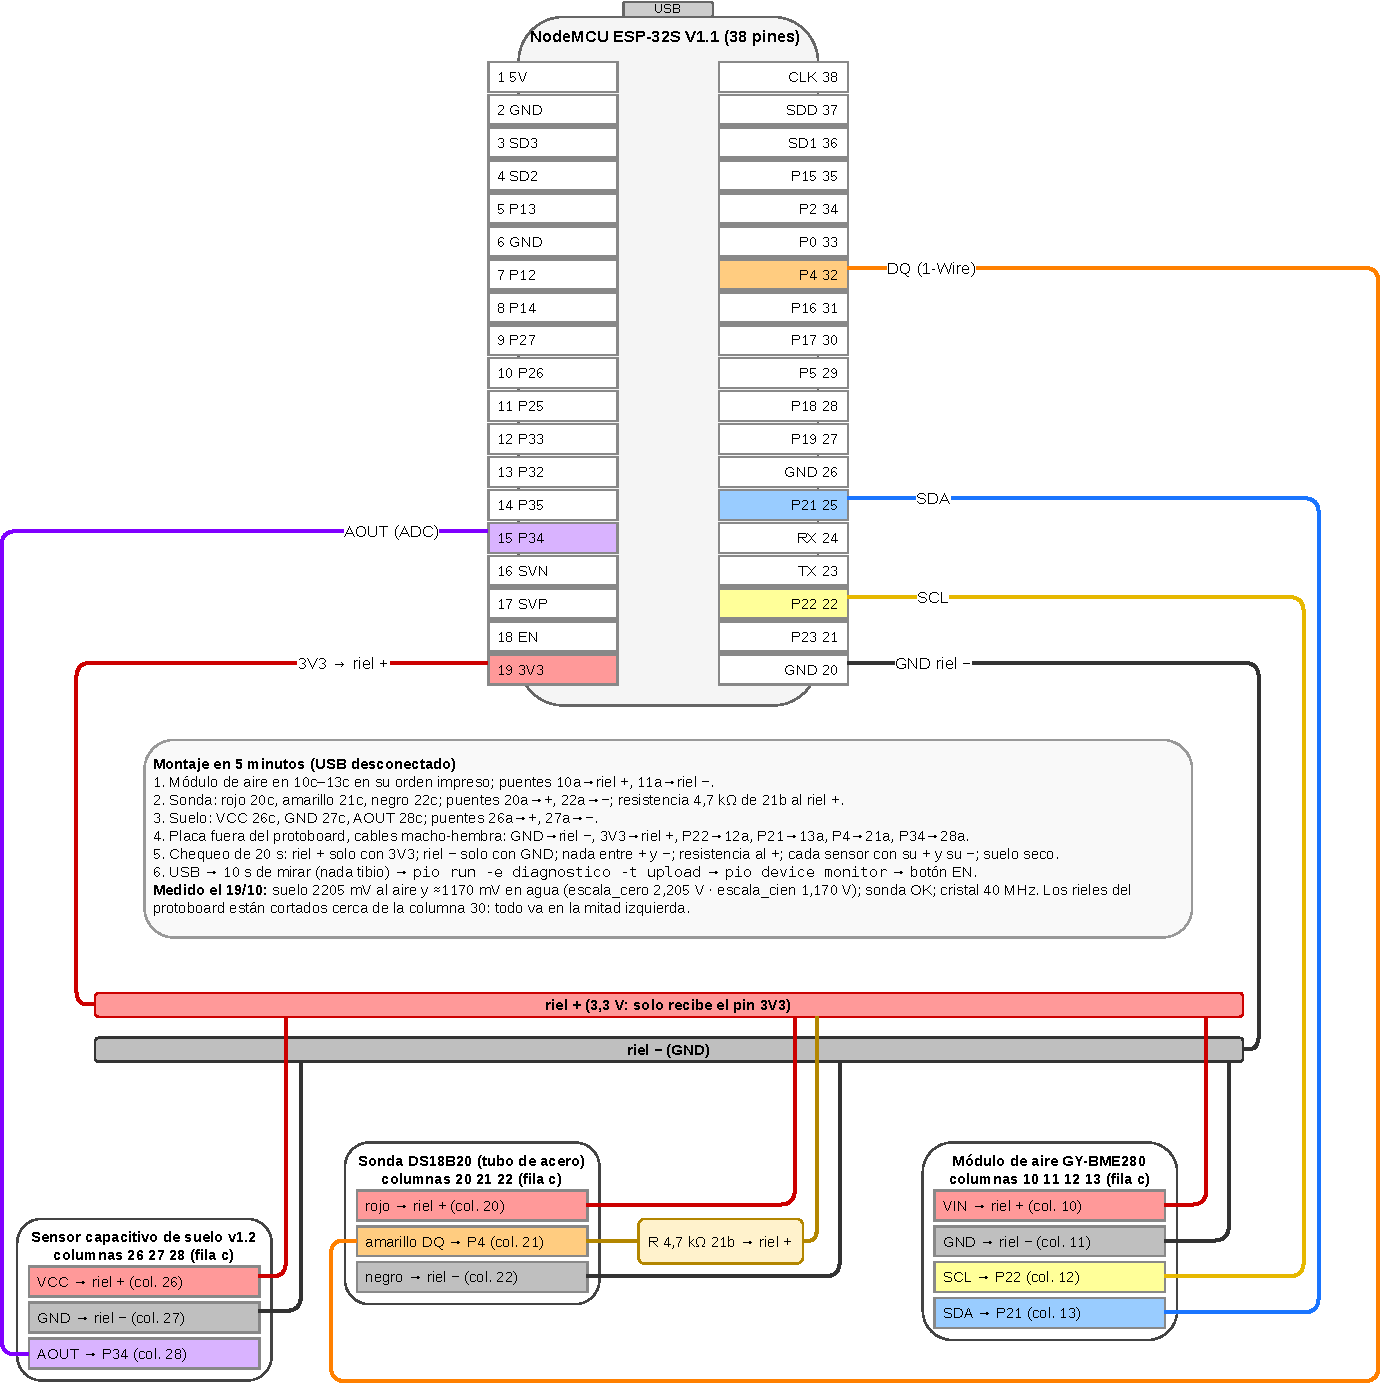
\includegraphics[width=\linewidth,height=0.86\textheight,keepaspectratio]{cableado-esp32.pdf}
    \end{column}
  \end{columns}
  \fuente{docs/17 §4.4; plataforma/firmware/cableado-fase-1.drawio (pines verificados contra el firmware)}
\end{frame}

\begin{frame}{Corrida de 24 h con el nodo propio (23--24/10)}
  \begin{columns}[T,onlytextwidth]
    \begin{column}{0.31\textwidth}\cifra{1\,440 de 1\,440}{tramas recibidas, una por minuto}\end{column}
    \begin{column}{0.31\textwidth}\cifra{0}{huecos de comunicación y reinicios}\end{column}
    \begin{column}{0.31\textwidth}\cifra{210}{tramas a cuarentena por una falla real del sensor}\end{column}
  \end{columns}
  \bigskip
  \begin{itemize}
    \item A las 15:24 falló el contacto I2C del sensor de aire: valores imposibles (183 °C y $-185$ hPa), todos a
      cuarentena con su motivo.
    \item La humedad de 100 \%, falsa pero dentro de lo posible, sí entró: es la lección de la lámina siguiente.
    \item Una prueba larga con hardware real destapa lo que ningún banco destapa.
  \end{itemize}
  \fuente{docs/16 §53}
\end{frame}

\begin{frame}{Lo que la corrida enseñó y ya está corregido}
  \begin{itemize}
    \item \textbf{Firmware:} omite el sensor que no responde (visto en la placa); el valor congelado, programado y por probar en la
      placa; watchdog de 120 s probado (dos cuelgues provocados, dos reinicios a los 120,0 s).
    \item \textbf{Plataforma:} vio esos dos cuelgues sola, sin saber nada del firmware: funciona con dispositivos que no
      controlamos.
    \item \textbf{Panel:} «canal callado»: el equipo reporta, pero una magnitud no llega.
    \item \textbf{Etapa 4 (iteración 2):} canal callado y valor congelado para \emph{cualquier} dispositivo, con lo declarado en el alta.
  \end{itemize}
  \fuente{docs/16 §53 y §54; docs/17}
\end{frame}

\begin{frame}{Servidor de prueba operando en la red del campus (desde el 03/11)}
  \footnotesize
  \begin{itemize}
    \item Equipo compartido con permiso; administración solo por red privada cifrada; un puerto hacia afuera (8883, TLS 1.2+).
    \item Verificado el 04/11: MQTT con TLS y HTTPS con token guardan; sin credencial, con credencial incorrecta, sin TLS y sin
      token, rechazado; TLS 1.1 fuera; 1883/3000/5432 cerrados.
    \item Respaldo diario con restauración probada; la pila se recupera sola al reiniciar sus contenedores ($\approx$ 1 min); el reinicio del equipo, por probar.
    \item Lo que falta: dirección de entrada desde Internet (pedida) y sesión de usuarios (bloque 1 de la Etapa 4).
  \end{itemize}
  \fuente{docs/14 §7.4; bitácora del 03--04/11}
\end{frame}

\begin{frame}[standout]
  Demostración del panel en vivo
\end{frame}

\begin{frame}{Rendimiento y consumo, medidos}
  \begin{columns}[T,onlytextwidth]
    \begin{column}{0.24\textwidth}\cifra{409/s}{pico de 30 s sin pérdida (RNF-01 pide 50/s; medido 59,7)}\end{column}
    \begin{column}{0.24\textwidth}\cifra{324 MiB}{pico de toda la pila (meta: 2 GB)}\end{column}
    \begin{column}{0.24\textwidth}\cifra{180 B}{por lectura en disco}\end{column}
    \begin{column}{0.24\textwidth}\cifra{0 de 180}{perdidas o duplicadas en cada entrada}\end{column}
  \end{columns}
  \footnotesize
  \begin{itemize}
    \item \textbf{50 tramas/s es una meta de estrés}, unas 300 veces la carga del campus (50 canales cada 5 min); la operación
      real es de una trama por nodo cada 60 s o más, y con ella se calcula el disco.
    \item El límite medido es la CPU de la base, no la memoria: 193 MiB en reposo (24/10). ThingsBoard CE pide 4 GB para una prueba
      de concepto.
    \item Mil nodos de 6 canales cada minuto usan $\approx$ 12 \% de lo medido; lo que manda es el disco.
  \end{itemize}
  \fuente{docs/02 (fundamento de RNF-01); docs/16 §10 y §49; docs/14 §2.1; docs/01 (referentes)}
\end{frame}

\begin{frame}{Costo de operación}
  \begin{columns}[T,onlytextwidth]
    \begin{column}{0.32\textwidth}
      \cifra{$\approx$ CLP 6\,000}{al mes: VPS de 2 vCPU y 4 GB}
      \cifra{$\approx$ 3 años}{100 nodos cada 5 min en 40 GB}
    \end{column}
    \begin{column}{0.64\textwidth}
      \begin{itemize}
        \item El costo no es fijo: \textbf{180 B $\times$ nodos $\times$ canales $\times$ lecturas al año}.
        \item La palanca es el intervalo, que se declara en el alta: 1\,000 nodos de 6 canales ocupan 568 GB al año a 60 s
          y 114 GB a 5 min.
        \item Precios del 10/09/2026.
      \end{itemize}
    \end{column}
  \end{columns}
  \fuente{docs/14 §2.1, §3 y §5}
\end{frame}

\begin{frame}{Avance de la Etapa 3 frente a la pauta}
  \small
  \begin{tabular}{@{}L{0.34\linewidth}L{0.6\linewidth}@{}}
    \toprule
    \textbf{Criterio (peso)} & \textbf{Estado} \\
    \midrule
    50 \% de implementación (10 \%) & \hecho: backlog completo 37 de 66 (56 \%); núcleo 25 de 34 (75 \%) y 4 parciales \\
    Pruebas iniciales (30 \%) & \avanzado: carga, carreras, TLS, capacidad, caídas, campo y 24 h; faltan TT-27 y el broker de producción \\
    Validación preliminar (10 \%) & \hecho: sensor real 24 h y red LoRaWAN real del campus (20/10); la del servidor, Etapa 4 \\
    Mejoras (15 \%) & \avanzado: decisiones del 6--8/10, proxy TLS, dependencias sin altas ni críticas \\
    Documentación (15 \%) & \hecho: informe y láminas con revisión final el 04/11 \\
    Retroalimentación (20 \%) & \encurso: entrevistas incorporadas; la de la Etapa 2, al recibirla \\
    \bottomrule
  \end{tabular}
  \fuente{docs/18 §1}
\end{frame}

\begin{frame}{Plan de la Etapa 4}
  \begin{columns}[T,onlytextwidth]
    \begin{column}{0.62\textwidth}
      \footnotesize
      \begin{enumerate}
        \item Seguridad, usuarios y roles (iteración 0).
        \item Panel para operar una flota, con alta masiva por archivo y bandeja de detectados (iteración 2).
        \item Salud de los datos: canal callado y valor congelado (iteraciones 1 y 2).
        \item Lo pedido en la entrevista del 05/10 (iteración 2).
        \item LoRaWAN completo: ruta C con ChirpStack externo, de punta a punta (iteración 0).
        \item Despliegue: servidor de prueba (iteración 0); Kubernetes, namespace ya medido, y consumo en pesos (iteración 2).
        \item Informe final (iteración 0); comparación completa con los referentes (iteración 2).
      \end{enumerate}
    \end{column}
    \begin{column}{0.33\textwidth}
      \cifra{$\approx$ 224 h}{de plan}
      \cifra{$\approx$ 75 h}{de presupuesto}
      \scriptsize Primero la iteración 0, el mínimo ($\approx$ 70 h, cabe en las 75); el resto por iteraciones, todo probado; lo que no alcance queda diseñado y declarado.
    \end{column}
  \end{columns}
  \fuente{docs/04 §8}
\end{frame}

\begin{frame}{Lo que necesito de usted}
  \begin{enumerate}
    \item Su retroalimentación sobre la Etapa 2 (pesa 20 \% en esta etapa).
    \item ¿Hay un ChirpStack institucional en el campus (ruta C), o la red sigue con la pasarela UG65 (ruta B)?
    \item La institución ya entregó un namespace de Kubernetes y un equipo compartido en la red del campus; falta una dirección
      de entrada desde Internet y cupo de volúmenes. ¿Nos ayuda a gestionarlo?
    \item ¿Le parece bien el orden de la Etapa 4, o algo debe subir?
  \end{enumerate}
\end{frame}

\appendix
\begin{frame}[plain]
  % Respaldo: la figura de contenedores del informe, si pide ver el detalle de las rutas LoRaWAN.
  \centering
  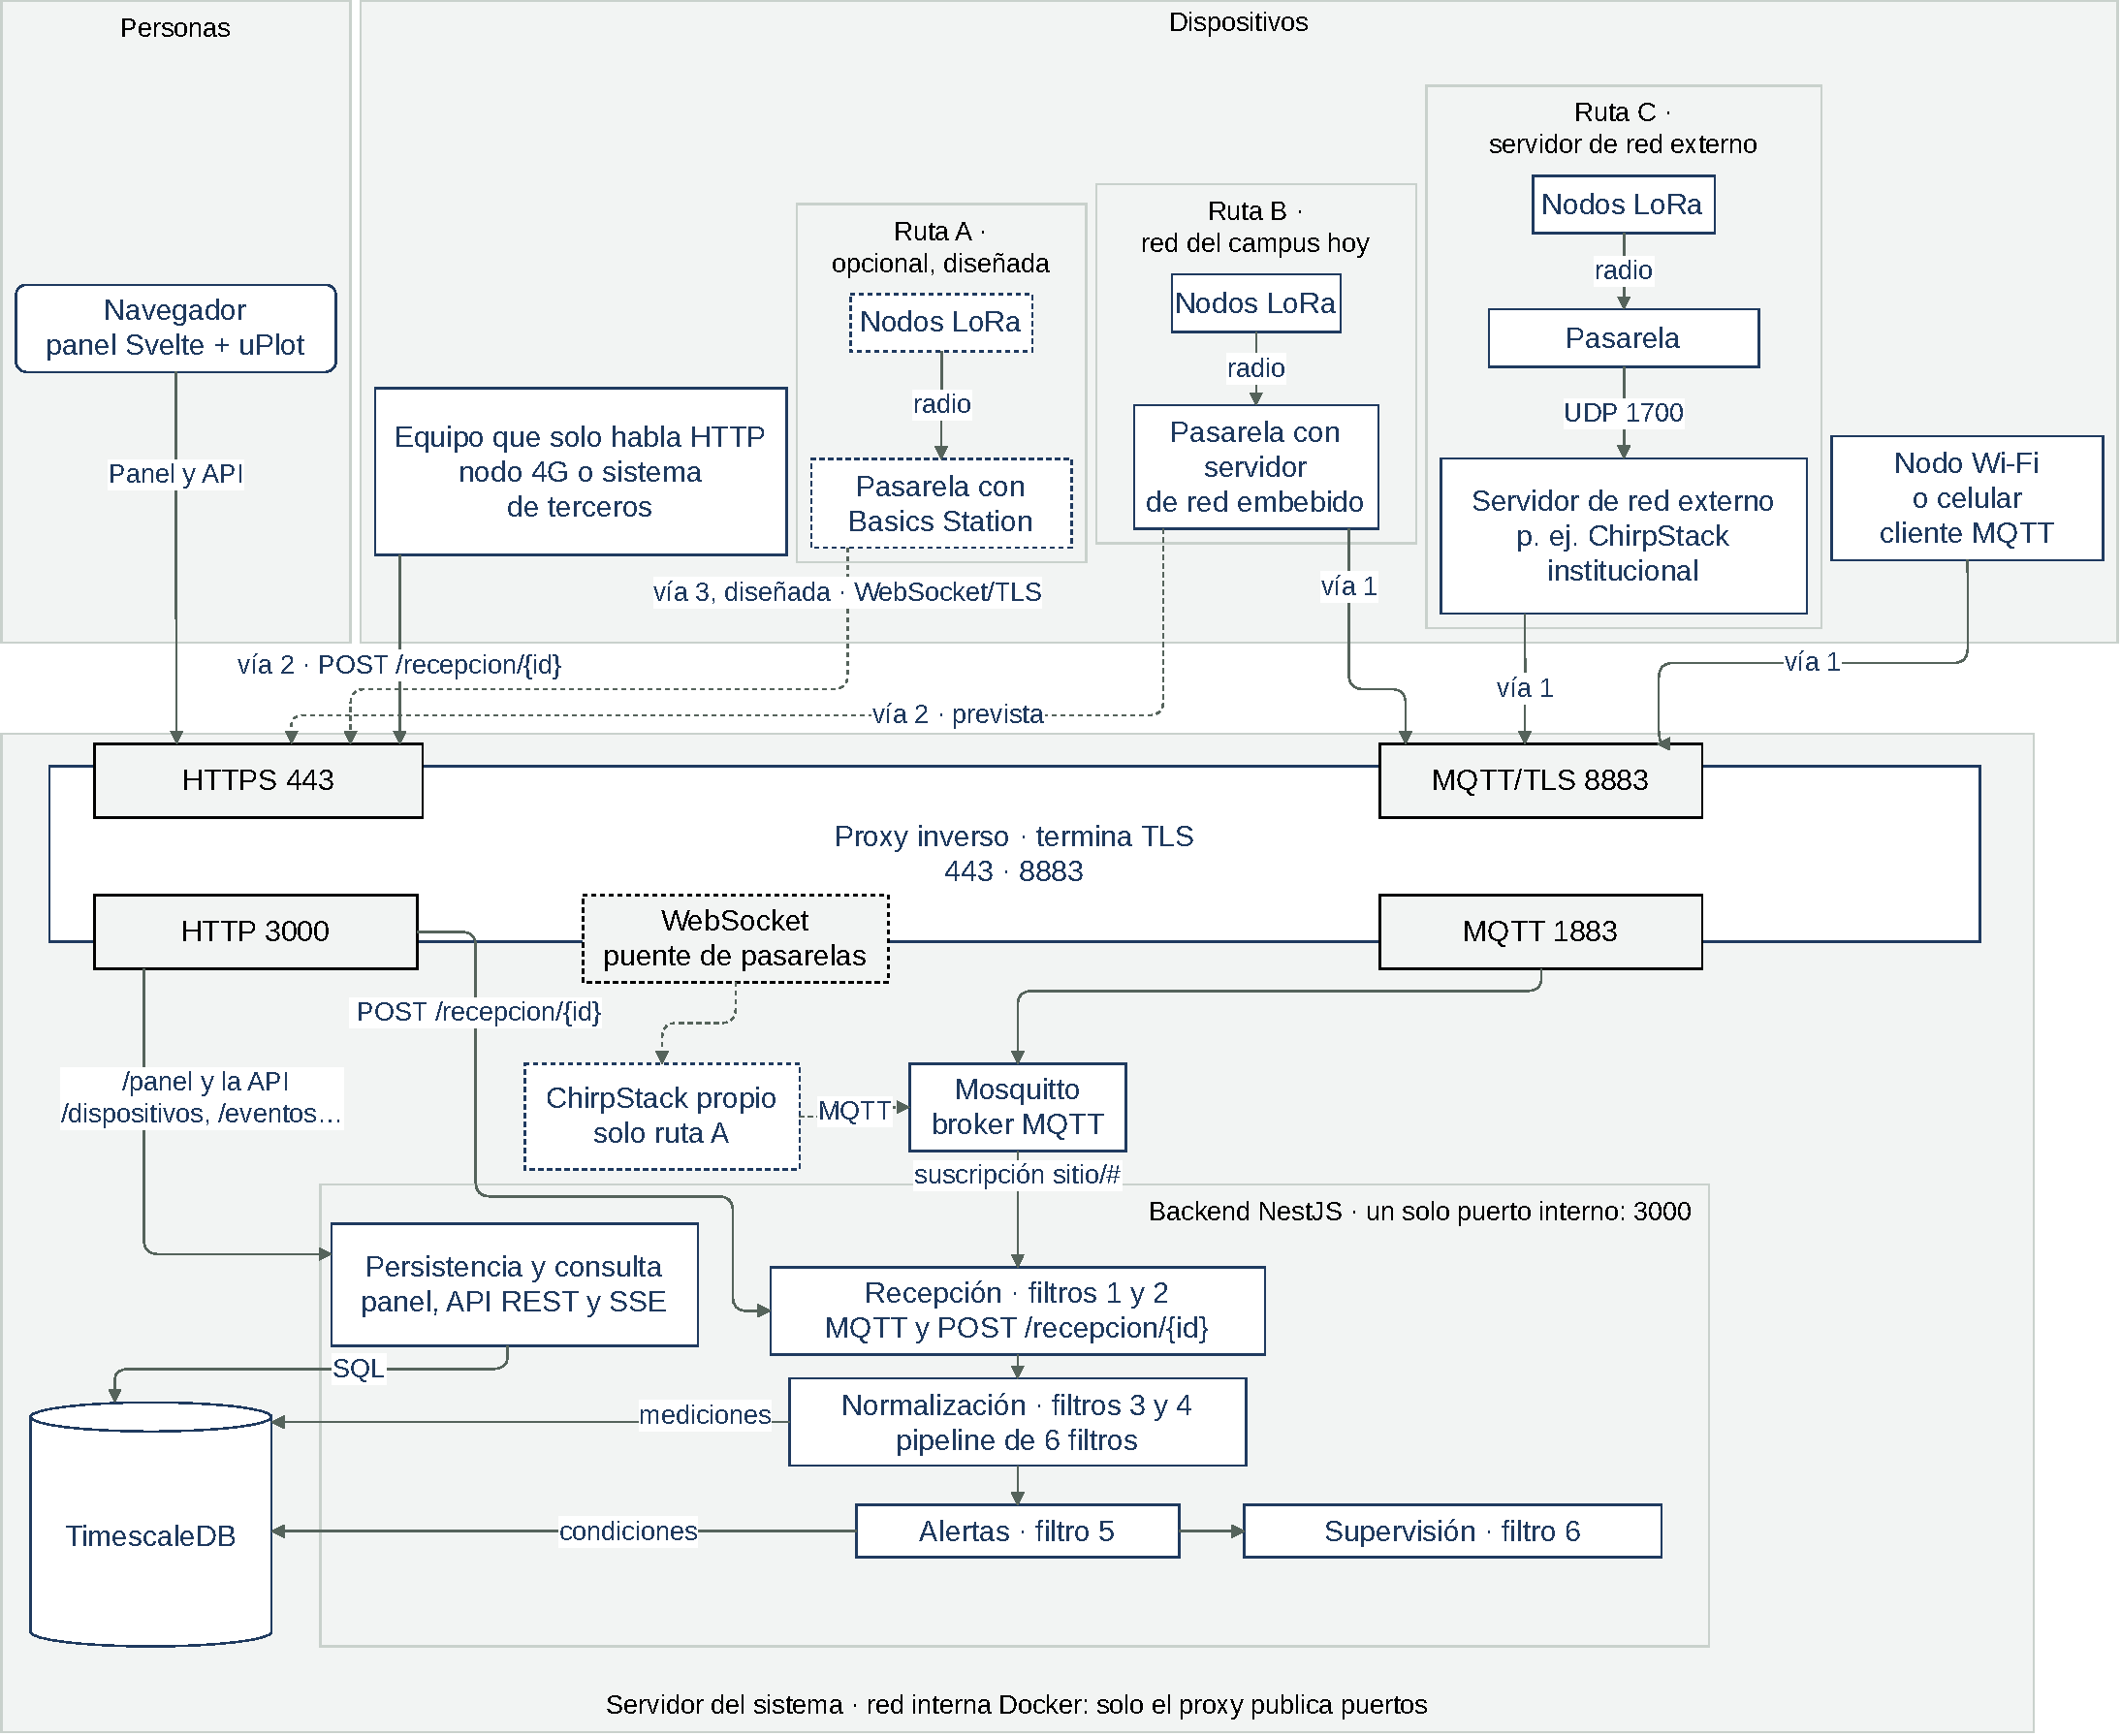
\includegraphics[width=\linewidth,height=0.94\textheight,keepaspectratio]{figura-4.1.pdf}
\end{frame}

\end{document}
